\subsubsection*{(c) Análise da matriz de confusão do Naive Bayes}

\begin{lstlisting}[language=Python]
cm = confusion_matrix(y_true=y_test, y_pred=yhats[0])
mask = 1 - np.identity(cm.shape[0])
error_matrix = np.multiply(cm, mask)

error_perc = error_matrix.sum(axis=1) / cm.sum(axis=1)

value, count = np.unique(y_train, return_counts=True)
\end{lstlisting}

\begin{figure}[H]
    \centering
    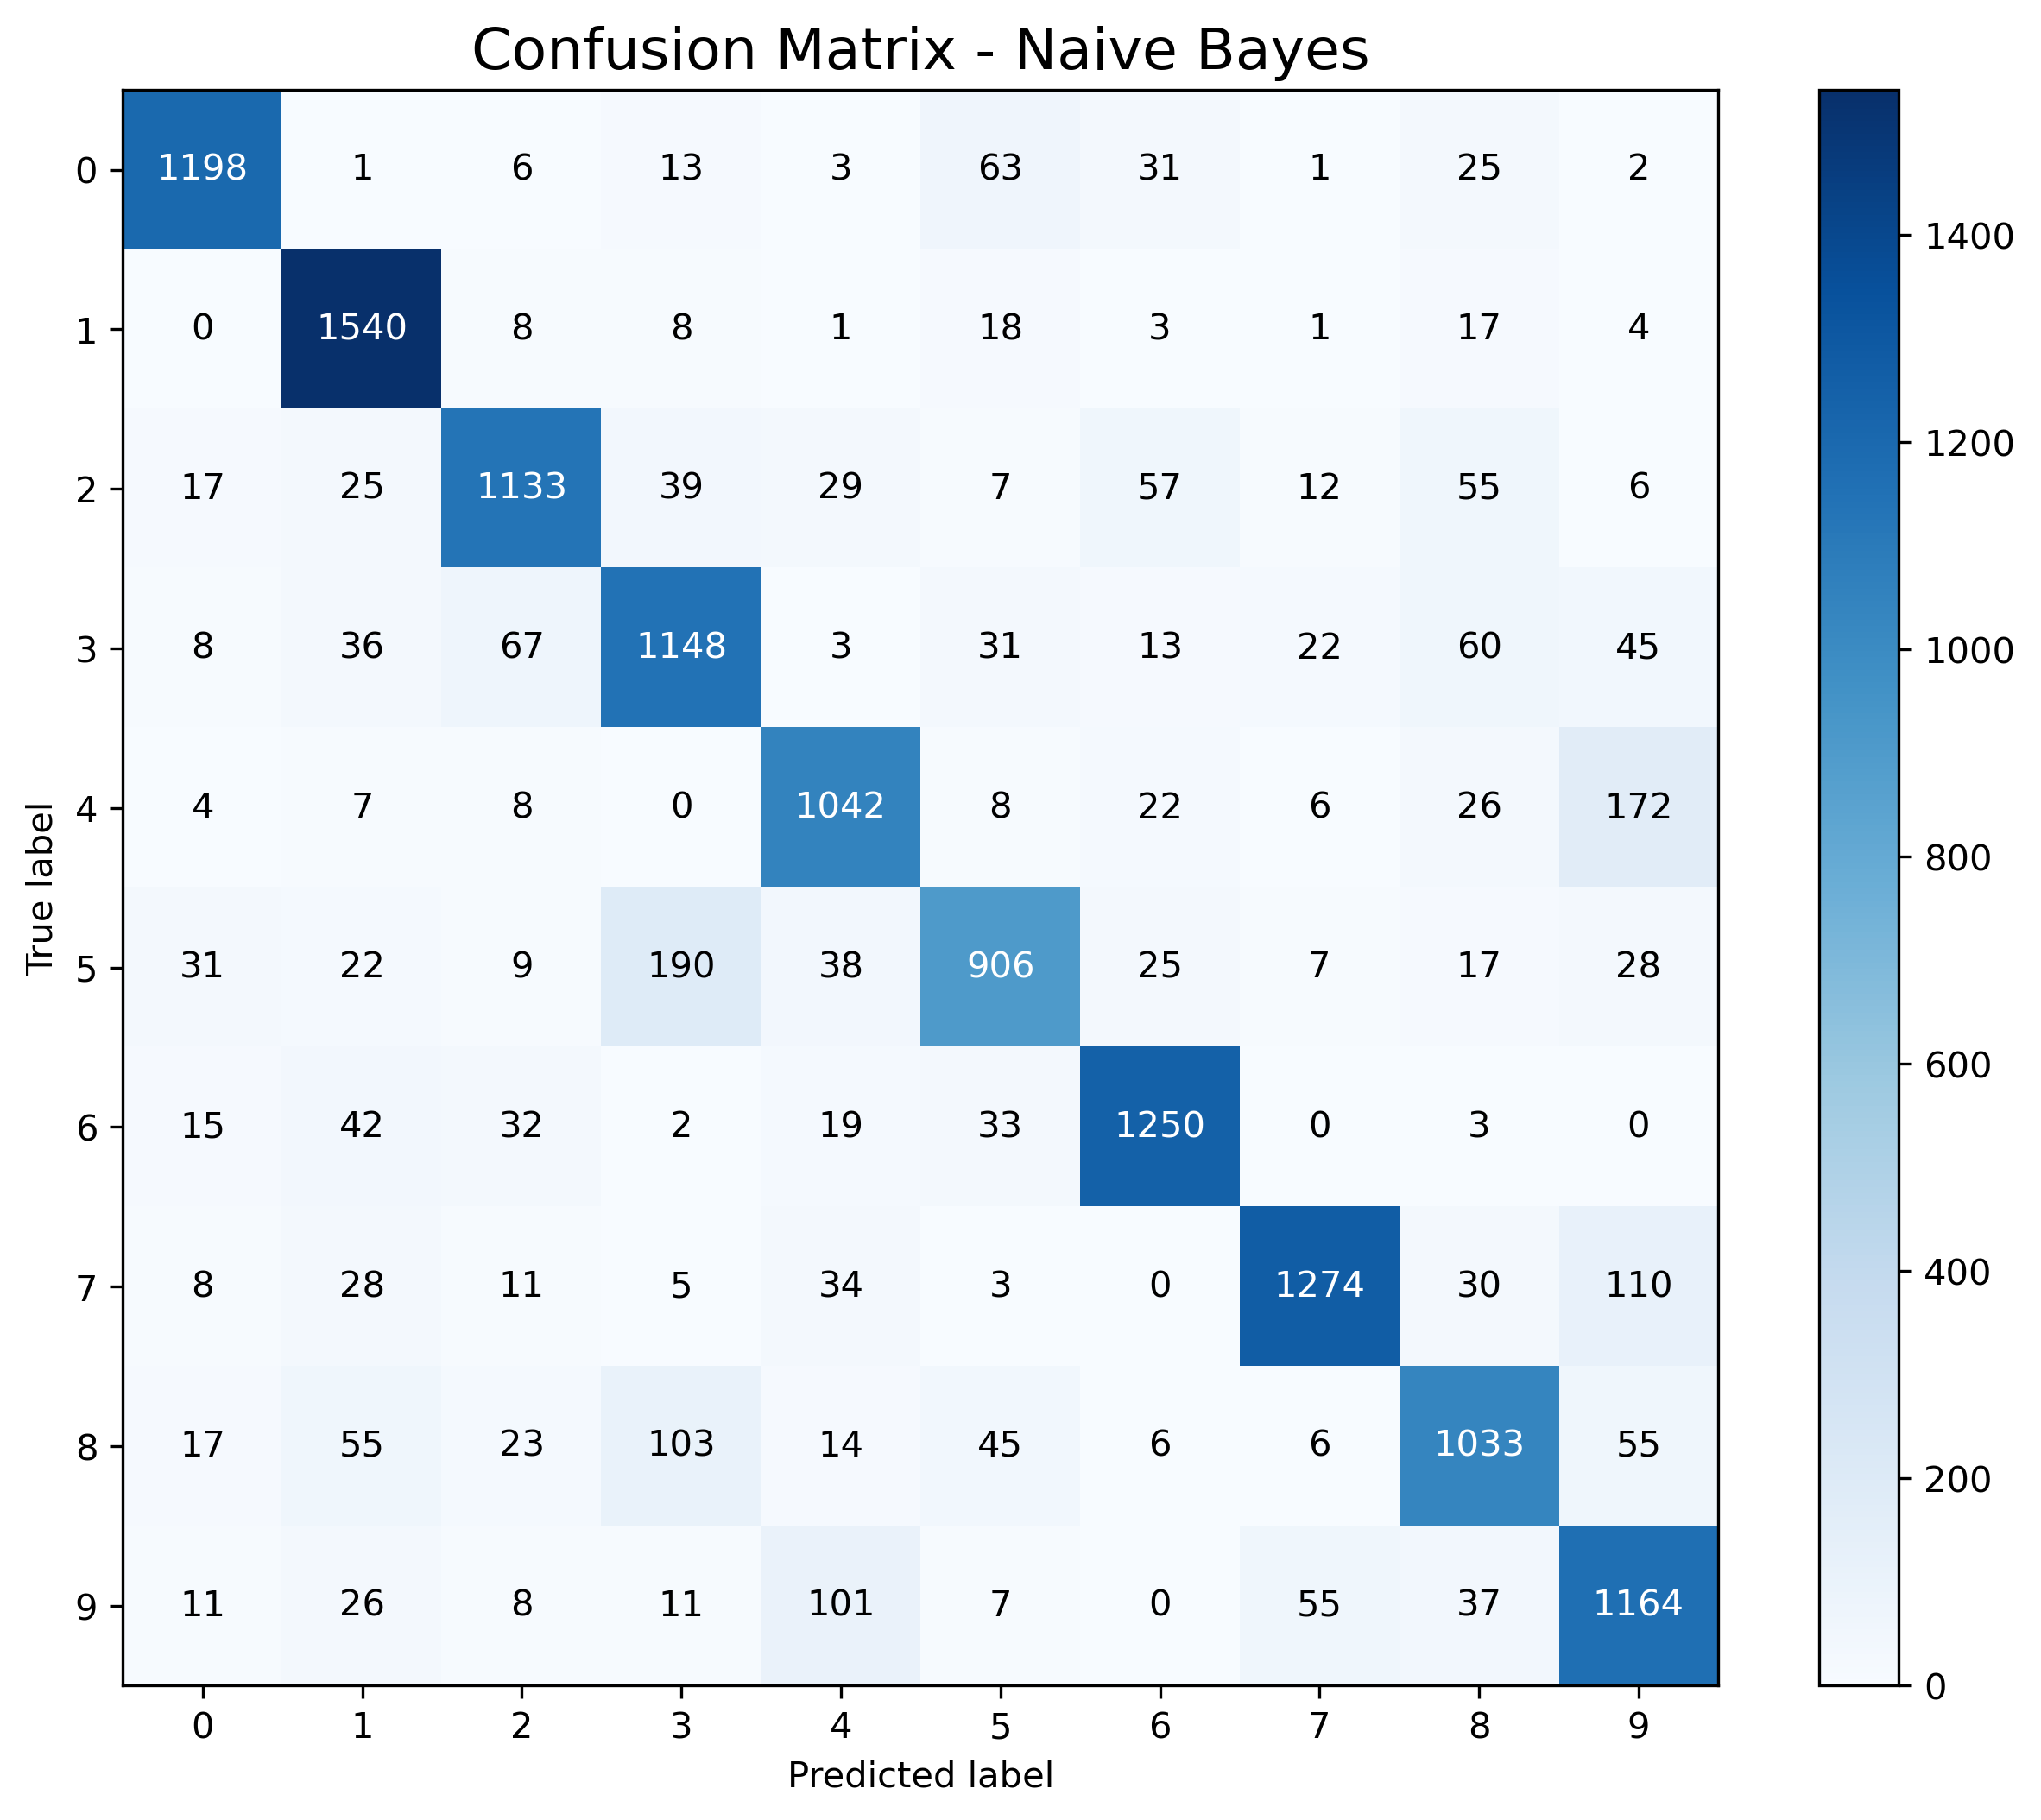
\includegraphics[width=0.8\textwidth]{../figures/3/confusion_matrix_naive_bayes.png}
    \caption{Matriz de confusão do modelo Naive Bayes}
    \label{fig:confusion_matrix}
\end{figure}

\textbf{Análise dos erros mais comuns:}

\begin{table}[H]
    \centering
    \begin{tabular}{|c|c|}
        \hline
        \textbf{Classe} & \textbf{Taxa de Erro (\%)} \\
        \hline
        0               & 10.8                       \\
        1               & 3.8                        \\
        2               & 17.9                       \\
        3               & 19.9                       \\
        4               & 19.5                       \\
        5               & 28.8                       \\
        6               & 10.5                       \\
        7               & 15.2                       \\
        8               & 23.9                       \\
        9               & 18.0                       \\
        \hline
    \end{tabular}
    \caption{Taxa de erro por classe no modelo Naive Bayes}
    \label{tab:error_rates}
\end{table}

A classe mais confundida foi a \textbf{5} (28.8\% de erro). Nota-se pela matriz de confusão que parte considerável dos erros para esta classe ocorreram pois o modelo previu \textbf{3, 0 e 8}. Provavelmente isso acontece pela semelhança visual dos dígitos \textbf{5, 3 e 8} e pelo desbalanceamento da classe \textbf{1} nos dados de treino, que foi a mais frequente (6.277 amostras).

\textbf{Contagem das classes nos dados de treino:}

\begin{table}[H]
    \centering
    \begin{tabular}{|c|c|c|c|c|c|c|c|c|c|c|}
        \hline
        \textbf{Classe}   & 0    & 1    & 2    & 3    & 4    & 5    & 6    & 7    & 8    & 9    \\
        \hline
        \textbf{Contagem} & 5560 & 6277 & 5610 & 5708 & 5529 & 5040 & 5480 & 5790 & 5468 & 5538 \\
        \hline
    \end{tabular}
    \caption{Distribuição das classes no conjunto de treinamento}
    \label{tab:class_distribution}
\end{table}